\documentclass[border=8pt]{standalone}
\usepackage[T1]{fontenc}
\usepackage{xcolor}
\usepackage{tikz}
\usetikzlibrary{arrows.meta, positioning}

% ---- Farben ----
\definecolor{tealfill}{HTML}{E1F5EE}
\definecolor{tealstroke}{HTML}{0F6E56}
\definecolor{tealtext}{HTML}{085041}

\definecolor{greenfill}{HTML}{EAF3DE}
\definecolor{greenstroke}{HTML}{3B6D11}
\definecolor{greentext}{HTML}{27500A}

\definecolor{amberfill}{HTML}{FAEEDA}
\definecolor{amberstroke}{HTML}{854F0B}
\definecolor{ambertext}{HTML}{633806}

\definecolor{grayfill}{HTML}{F1EFE8}
\definecolor{graystroke}{HTML}{5F5E5A}
\definecolor{graytext}{HTML}{444441}

\definecolor{coralfill}{HTML}{FAECE7}
\definecolor{coralstroke}{HTML}{993C1D}
\definecolor{coraltext}{HTML}{712B13}

% ---- Maße ----
\newcommand{\boxw}{6.0cm}      % einheitliche Breite aller rechten Kästen
\newcommand{\boxh}{1cm}        % einheitliche Höhe aller rechten Kästen

% ---- Node-Styles ----
\tikzset{
    proc/.style={rectangle, rounded corners=3pt, draw=tealstroke, fill=tealfill,
    minimum width=3.2cm, minimum height=1cm, align=center, font=\small},
    greenbox/.style={rectangle, rounded corners=3pt, draw=greenstroke, fill=greenfill,
    minimum width=\boxw, minimum height=\boxh, align=center, font=\small},
    kernelbox/.style={rectangle, rounded corners=3pt, draw=amberstroke, fill=amberfill,
    line width=1pt, minimum width=\boxw, minimum height=\boxh, align=center, font=\small},
    grayhdr/.style={rectangle, rounded corners=3pt, draw=graystroke, fill=grayfill,
    minimum width=3.2cm, minimum height=1cm, align=center, font=\small},
    greenhdr/.style={rectangle, rounded corners=3pt, draw=graystroke, fill=grayfill,
    minimum width=\boxw, minimum height=\boxh, align=center, font=\small},
    entfaellt/.style={rectangle, rounded corners=3pt, draw=graystroke, fill=grayfill,
    dashed, minimum width=\boxw, align=center, font=\small, text=graytext},
    note/.style={rectangle, rounded corners=5pt, draw=coralstroke, fill=coralfill,
    minimum width=\boxw, align=center, font=\footnotesize, text=coraltext, inner sep=4pt},
    lifeline/.style={dashed, gray, thin},
    arrbig/.style={-{Latex[length=2.5mm]}, thick},
}

\begin{document}
    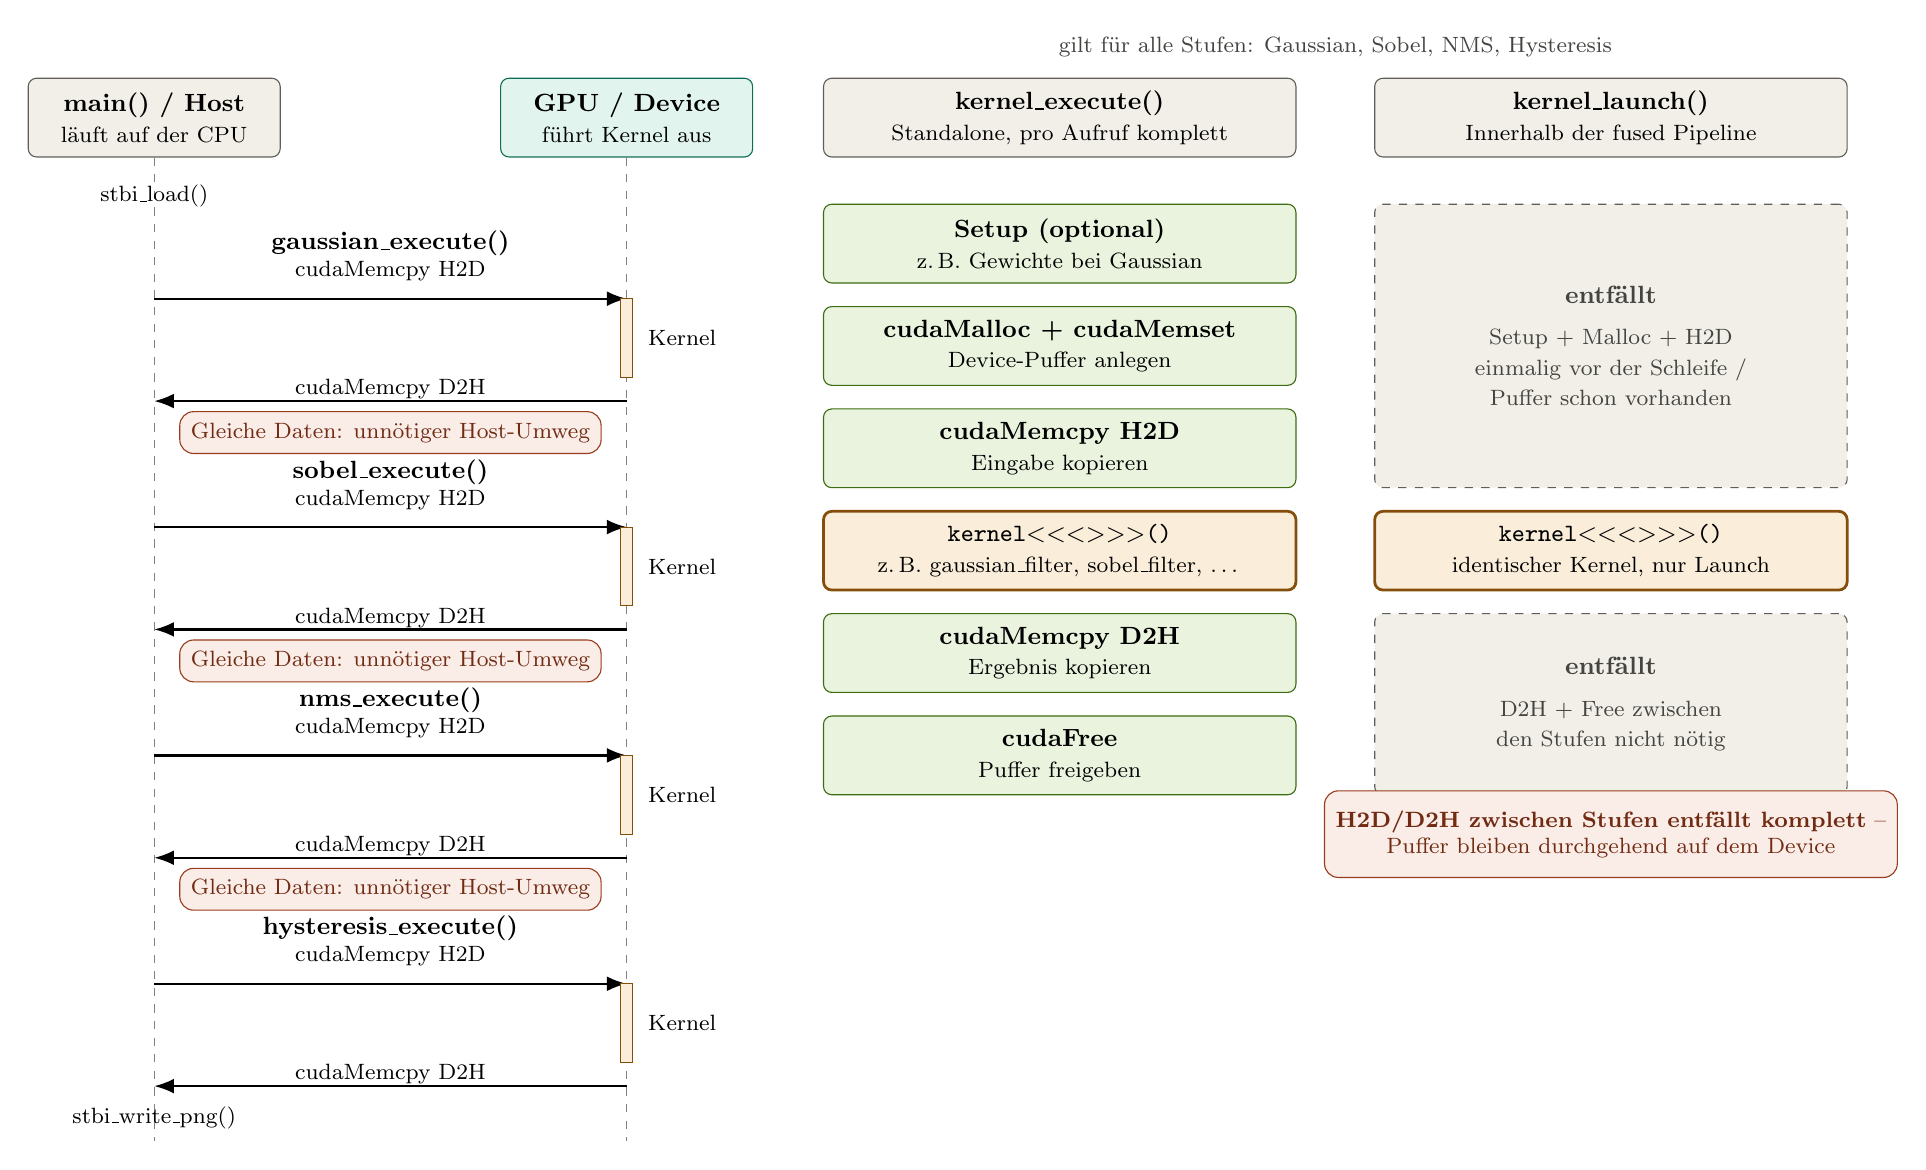
\begin{tikzpicture}[y=1cm, x=1cm]

% =========================================================
% LEFT PANEL — Sequence diagram
% =========================================================

        \node[grayhdr] (host) at (0, 0) {\textbf{main() / Host}\\{\footnotesize läuft auf der CPU}};
        \node[proc]    (gpu)  at (6, 0) {\textbf{GPU / Device}\\{\footnotesize führt Kernel aus}};

        \draw[lifeline] (host) -- ++(0,-13.0);
        \draw[lifeline] (gpu)  -- ++(0,-13.0);

% stbi_load() direkt auf der Lifeline, wie stbi_write_png() unten
        \node[font=\footnotesize] at (0,-1.0) {stbi\_load()};

% Stage 1: Gaussian
        \node[font=\small\bfseries] at (3,-1.6)  {gaussian\_execute()};
        \node[font=\footnotesize]   at (3,-1.95) {cudaMemcpy H2D};
        \draw[arrbig] (0,-2.3) -- (6,-2.3);
        \draw[fill=amberfill, draw=amberstroke] (5.925,-2.3) rectangle (6.075,-3.3);
        \node[font=\footnotesize, anchor=west] at (6.15,-2.8) {Kernel};
        \node[font=\footnotesize] at (3,-3.45) {cudaMemcpy D2H};
        \draw[arrbig] (6,-3.6) -- (0,-3.6);
        \node[note, minimum width=5cm] at (3,-4.0) {Gleiche Daten: unnötiger Host-Umweg};

% Stage 2: Sobel
        \node[font=\small\bfseries] at (3,-4.5)  {sobel\_execute()};
        \node[font=\footnotesize]   at (3,-4.85) {cudaMemcpy H2D};
        \draw[arrbig] (0,-5.2) -- (6,-5.2);
        \draw[fill=amberfill, draw=amberstroke] (5.925,-5.2) rectangle (6.075,-6.2);
        \node[font=\footnotesize, anchor=west] at (6.15,-5.7) {Kernel};
        \node[font=\footnotesize] at (3,-6.35) {cudaMemcpy D2H};
        \draw[arrbig] (6,-6.5) -- (0,-6.5);
        \node[note, minimum width=5cm] at (3,-6.9) {Gleiche Daten: unnötiger Host-Umweg};

% Stage 3: NMS
        \node[font=\small\bfseries] at (3,-7.4)  {nms\_execute()};
        \node[font=\footnotesize]   at (3,-7.75) {cudaMemcpy H2D};
        \draw[arrbig] (0,-8.1) -- (6,-8.1);
        \draw[fill=amberfill, draw=amberstroke] (5.925,-8.1) rectangle (6.075,-9.1);
        \node[font=\footnotesize, anchor=west] at (6.15,-8.6) {Kernel};
        \node[font=\footnotesize] at (3,-9.25) {cudaMemcpy D2H};
        \draw[arrbig] (6,-9.4) -- (0,-9.4);
        \node[note, minimum width=5cm] at (3,-9.8) {Gleiche Daten: unnötiger Host-Umweg};

% Stage 4: Hysteresis
        \node[font=\small\bfseries] at (3,-10.3)  {hysteresis\_execute()};
        \node[font=\footnotesize]   at (3,-10.65) {cudaMemcpy H2D};
        \draw[arrbig] (0,-11.0) -- (6,-11.0);
        \draw[fill=amberfill, draw=amberstroke] (5.925,-11.0) rectangle (6.075,-12.0);
        \node[font=\footnotesize, anchor=west] at (6.15,-11.5) {Kernel};
        \node[font=\footnotesize] at (3,-12.15) {cudaMemcpy D2H};
        \draw[arrbig] (6,-12.3) -- (0,-12.3);

        \node[font=\footnotesize] at (0,-12.7) {stbi\_write\_png()};

% =========================================================
% RIGHT PANEL — gaussian_execute() vs gaussian_launch()
% Deutlich mehr Abstand zum linken Panel, kein Trenner-Strich
% =========================================================

        \def\colA{11.5}
        \def\colB{18.5}

        \node[greenhdr] (h1) at (\colA, 0) {\textbf{kernel\_execute()}\\{\footnotesize Standalone, pro Aufruf komplett}};
        \node[greenhdr] (h2) at (\colB, 0) {\textbf{kernel\_launch()}\\{\footnotesize Innerhalb der fused Pipeline}};
        \node[font=\footnotesize, text=graytext] at (15, 0.9) {gilt für alle Stufen: Gaussian, Sobel, NMS, Hysteresis};

        \node[greenbox] (r1) at (\colA,-1.6) {\textbf{Setup (optional)}\\{\footnotesize z.\,B. Gewichte bei Gaussian}};
        \node[greenbox] (r2) at (\colA,-2.9) {\textbf{cudaMalloc + cudaMemset}\\{\footnotesize Device-Puffer anlegen}};
        \node[greenbox] (r3) at (\colA,-4.2) {\textbf{cudaMemcpy H2D}\\{\footnotesize Eingabe kopieren}};
        \node[kernelbox] (r4) at (\colA,-5.5) {\textbf{\texttt{kernel}}$<<<>>>$\textbf{\texttt{()}}\\{\footnotesize z.\,B. gaussian\_filter, sobel\_filter, \ldots}};
        \node[greenbox] (r5) at (\colA,-6.8) {\textbf{cudaMemcpy D2H}\\{\footnotesize Ergebnis kopieren}};
        \node[greenbox] (r6) at (\colA,-8.1) {\textbf{cudaFree}\\{\footnotesize Puffer freigeben}};

        \node[entfaellt, minimum height=3.6cm] (topskip) at (\colB,-2.9)
            {\textbf{entfällt}\\[4pt]{\footnotesize Setup + Malloc + H2D}\\{\footnotesize einmalig vor der Schleife /}\\{\footnotesize Puffer schon vorhanden}};

        \node[kernelbox] (r4b) at (\colB,-5.5) {\textbf{\texttt{kernel}}$<<<>>>$\textbf{\texttt{()}}\\{\footnotesize identischer Kernel, nur Launch}};

        \node[entfaellt, minimum height=2.3cm] (botskip) at (\colB,-7.45)
            {\textbf{entfällt}\\[4pt]{\footnotesize D2H + Free zwischen}\\{\footnotesize den Stufen nicht nötig}};

        \node[note, minimum height=1.1cm] at (\colB,-9.1)
            {\textbf{H2D/D2H zwischen Stufen entfällt komplett} --\\Puffer bleiben durchgehend auf dem Device};

    \end{tikzpicture}
\end{document}